\section[连续时间中的随机过程]{连续时间中的随机过程\\Random Processes in Continuous Time}
	\subsection{Random Processes in Continuous Time}
	So far the order of observations has been of no concern. We collected all the observations and by least squares we estimated the parameters in $ x $.However, The time for the observation does play a role. The observation made at time t is denoted $ x(t) $.The sequence of observations taken at times$ t=t_{1},t_{2}...t_{n} $is denoted $ x(t_{1}),x(t_{2}),x(t_{n}) $.We are observing(and then estimating) a function of time.
	
	 Unavoidably there are errors in the observations. Each observation is a random variable and the whole sequence $ x(t) $ ,$ t=t_{1},t_{2}...t_{n} $ is a random process.A process is the evolution over time of a dynamic system. We must and shall develop a statistical theory for these functions. Classical statistical theory aims to infer the probability law of a random variable $ x $from a finite number of independent observations $ x_{1},x_{2}...x_{n} $. In this chapter we are observing a function that changes with time. We have a probability distribution for functions. 
	 
	 The system consisting of the Earth and a GPS satellite is an example of a dynamic system. Their motions are governed by laws that depend only on current relative positions and velocities. Such dynamic systems are often modeled by differential equations. We solve differential equations to obtain formulas for predicting the future behavior of dynamic systems. 
	 
	 The vector $ x(t) $ is the state of the process.The original process $ b(t) $ is required to be a linear combination of the system variables via $ b(t)=A(t)x(t)+e(t) $.
	 
	 Except for this error $ e(t) $, the process $ b(t) $ can be recovered from the model $ x(t) $ by a linear combination of state variables. 
	 
	  A linear random process in continuous time with state $ x(t) $  and state covariance $ \sum(t) $ has the model equations
	  
	  \begin{equation}\label{5.1}
	   \dot{x}(t)=F(t)x(t)+G(t)\varepsilon(t)
	  \end{equation}
	  
	  \begin{equation}\label{5.2}
	  \dot{b}(t)=A(t)x(t)+e(t)
	  \end{equation}
	  
	  \begin{equation}\label{5.3}
	  \dot{\sum}(t)=F(t)\sum(t)+\sum(t)F^{T}(t)+G(t)\sum\nolimits_{\epsilon}(t)G^{T}(t)
	  \end{equation}
	  
	  
	   
	  
	   The observation noise is measured by $ e(t) $ and the system noise by $ \varepsilon(t) $ with covariance $ \sum \varepsilon (t) $. Often initial values for the state are given.
	   
	   \textbf{Example 5.1} (Random ramp) A process with random initial value $ a_{0} $  and random slope $ a_{1} $ may be written as 
	   
	   \begin{equation}\label{5.4}
	    b(t)=a_{0}+a_{1}t \quad(5.4)
	   \end{equation}
	  
	   
	     The differential equation corresponding to (5.4) is
	     
	    $\ddot{b}(t)=0  $ with initial conditions $ b(0)=a_{0} $  and $ \dot{b}(0)=a_{1} $ 
	    
	    This is a second order differential equation so the state vector $ x $ for the process $ b $ must have two components. The dimension of the state vector equals the number of degrees of freedom of the system. Using phase variables $ x(t)=(x_{1},x_{2})=(b(t),\dot{b}(t)) $in the vector model leads to
	    
	    \[ \begin{bmatrix} \dot{x_{1}}  \\ \dot{x_{2}} \end{bmatrix} \quad=\begin{bmatrix} 0 & 1 \\ 0 &  0 \end{bmatrix} \quad\begin{bmatrix} x_{1}  \\ x_{2}  \end{bmatrix} \quad+\begin{bmatrix} 0 \\ 0 \end{bmatrix} \quad\epsilon\] 
	    \[ \begin{bmatrix} x_{1}(0)\\ x_{2}(0)\ \end{bmatrix} \quad=\begin{bmatrix} a_{0} \\ a_{1}\end{bmatrix} \quad \]
	    \[ b= \begin{bmatrix} 1 & 0\end{bmatrix} \quad\begin{bmatrix} x_{1}\\ x_{2}\ \end{bmatrix} \quad+e(t)\]
	    
	    Frequently random errors exhibit a definite time-growing behavior. A function which grows linearly with time can be used to describe them. The growth rate $ a1 $ is a random quantity with a given probability density.Two state elements are necessary to describe the model which is called a random ramp: 
	    \begin{equation}\label{5.5}
	    \dot{x_{1}}=x_{2}\quad and \quad \dot{x_{2}}=0
	    \end{equation}
	   
	    
	    The state $ x_{1} $ is the random ramp process; $ x_{2} $ is an auxiliary variable whose initial condition provides the slope of the ramp.The solution of (5.5) is $ x_{1}(t)=tx_{2}(0) $. The variance of $ x_{1} $ is seen to grow quadratically with time.So the covariance matrix is
	    
	   $ \sum(t)=\begin{bmatrix} t^{2}\sigma^{2} & t\sigma^{2} \\ t\sigma^{2} & \sigma^{2} \end{bmatrix} \quad $  hence   $ \dot{\sum}(t)=\begin{bmatrix} 2t^{2}\sigma^{2} & \sigma^{2} \\ \sigma^{2} & 0 \end{bmatrix} \quad  $ 
	   
	   We want to check this result by means of equation (5.3)
	   
	   \subsection {Mean and Correlation}  
	  In analogy with a single random variable we define the mean of an n-dimensional random process. The mean is a vector $ \mu $:
	  \begin{equation}\label{5.6}
	  E\left\lbrace  x(t)\right\rbrace  =\mu=\int_{-\infty}^{+\infty}x(t)p(x(t))dt
	  \end{equation}
	 
	  
	  Or component-wise
	  \begin{equation}\label{5.7}
	   E\left\lbrace  x_{i}(t)\right\rbrace  =\mu_{i}=\int_{-\infty}^{+\infty}x_{i}(t)p(x(t))dt,i=1,2...n
	  \end{equation}
	  
	  
	  A random process is called Gaussian or normal if its probability density function is normal. The autocorrelation function for a random process $ x(t) $ is defined as the expected value of the product $ x(t_{1})x(t_{2})^{T} $
	  \begin{equation}\label{5.8}
	   Autocorrelation \quad R_{x}(t_{1},t_{2}) =E\left\lbrace x(t_{1})x(t_{2})^{T}\right\rbrace 
	  \end{equation}
	  
	  
	  where $ t_{1} $ and $ t_{2} $ are arbitrary observation times. Sometimes you find the correlation properties of a random process described by means of the autocovariance function which is defined as . The two functions are obviously related. The mean is included in the autocorrelation and the mean is subtracted in the autocovariance $ E\left\lbrace(x(t_{1})-u(t_{1}))(x(t_{2})-u(t_{2}))^{T} \right\rbrace  $. The two functions are identical for processes with zero mean. 
	  
	  The autocorrelation tells how well the process is correlated with itself at two different times. A rapidly decreasing autocorrelation function has a “short memory” and allows the process to jump. A function with “long memory” entails a more smooth process.
	  
	   \subsubsection { Stationarity} 
	   
	   A random process is stationary if the density functions $ p(x(t)) $describing the process are invariant under translation of time.This means that 
	   
	   \[ p(x(t_{1})) = p(x(t_{1}+t))  \]
	   
	   in this stationary case the autocorrelation function depends only on the time difference $ \tau=t_{2}-t_{1} $ . Thus $ R_{x} $ reduces to a function of just one variable $ \tau $ :
	   \begin{equation}\label{5.9}
	   stationarity \quad autocorrelation \quad R_{x}(\tau) = E\{x(t)x(t+\tau)^{T}\}
	   \end{equation}
	     
	   
	   Stationarity assures us that the expectation does not depend separately on $ t_{1}=t $ and $ t_{2}=t+\tau $ ,but only on the difference $ \tau $ .
	   
	   \textbf{Example 5.2} (Random walk) The process is the result of integrating uncorrelated signals. The name indicates fixed-length steps in arbitrary directions. When the number of steps $ n $ is large and the individual steps are short, the distance travelled in a particular direction resembles the random walk process. 
	   
	   The random walk then is described as $ x(t_{n}=l_{1}+l_{2}+...l_{n}) $ . By linearity the mean value is $ E\left\lbrace x(t)\right\rbrace = 0  $ ,Let each $ l_{i} $ have variance $ \sigma_{i}^{2}=1 $.Independent steps yield 
	   
	   \[ Var(x(t_{n})) =1+1+1...+1=n\]
	   
	   For $ n\rightarrow\infty $ the variance of $ x $ tends to $ \infty $, so the process is not stationary! For the autocorrelation we have
	   \begin{equation}\label{5.10}
	    R_{x}(t_{1},t_{2}) = E\left\lbrace x(t_{1})x(t_{2})\right\rbrace =\int_{0}^{t_{2}}\int_0^{t_{1}} \delta(\tau-\sigma)d\tau d\sigma=\{_{t1,for t_{1} < t_{2}}^{t_{2},for t_{1} > t_{2}} 
	   \end{equation}
	    
	   
	   The continuous random walk process is also known as the Wiener process. The Wiener process defined by (5.10) is often taken as the definition of the white noise process. So Gaussian white noise is that hypothetical process, when integrated, which yields a Wiener process. See also Example 5.6. 
	   
	                
	   \subsubsection { Cross correlation} 
	   
	   Suppose we have two random processes $ x(t) $ and $ y(t) $. Their cross correlation function gives the expected values of all the products $ x_{i}(t_{1})y_{j}(t_{2}) $In matrix form:
	   \begin{equation}\label{5.11}
	    R_{xy}(t_{1},t_{2}) = E\left\lbrace x(t_{1}y(t_{2}^{T})) \right\rbrace
	   \end{equation}
	   
	    
	    If both processes are stationary,only the time difference $ \tau=t_{2}-t_{1} $ between sample points is relevant. We again have a (matrix) function of $ r $ alone:
	    \begin{equation}\label{5.12}
	     R_{xy}(\tau) = E\left\lbrace x(t)y(t+\tau)) \right\rbrace 
	    \end{equation}
	   
	    
	    The cross correlation function gives information on the mutual correlation between the two processes. Note that $ R_{xy}(\tau)=R_{yx}(-\tau) $ . The sum of two stationary random processes $ \tau(t)=x(t)+y(t) $ has an autocorrelation function defined as 
	    
	    
	    \begin{equation}\label{5.13}
	    \begin{aligned}
	     R_{Z}(\tau)&=E\left\lbrace (x(t)+y(t))(x(t+\tau)+y(t+\tau))^{T}\right\rbrace\\
	     &=E\left\lbrace x(t)x(t+\tau)^{T}\right\rbrace +E\left\lbrace x(t)y(t+\tau)^{T}\right\rbrace\\
	     &\quad +E\left\lbrace y(t)x(t+\tau)^{T}\right\rbrace+E\left\lbrace y(t)y(t+\tau)^{T}\right\rbrace \\
	     &=R_{x}(\tau)+R_{xy}(\tau)+R_{yx}(\tau) +R_{y}(\tau)
	    \end{aligned}  
	    \end{equation}
	    
	    
	    If $ x $ and $ y $ are uncorrelated processes with zero mean, then $ Rxy =0 $ and $ Ryx=0 $ and 
	    \begin{equation}\label{5.14}
	    R_{Z}(\tau)=R_{x}(\tau)+R_{y}(\tau) 
	    \end{equation}
	     
	    
	    The sum can be extended to more stationary and uncorrelated processes. We summarize some properties for stationary processes with zero mean: 
	    
	    1  $ R_{x}(0) $ is the mean-square value of the process  $x(t)$. 
	    
	    2  $ R_{x}(\tau) $ is an even function:$  R_{x}(\tau)= R_{x}(-\tau) $ .This follows from stationarity. 
	    
	    3 $ \left|R_{x}(\tau) < R_{x}(0) \right|  $ for all $ \tau $ . The mean-square value of $x(t)$ equals that of $x(t+r)$ .The correlation coefficient between these two random variablesis never greater than unity, by the Schwarz inequality. 
	    
	    4  If $ x(t)$ contains no periodic component,then  $R_{x}(\tau)$ tends to zero as $t\rightarrow\infty$.Therefore $x(t + r)$ becomes uncorrelated with $x(t)$ for large $\tau$ , provided there are no hidden periodicities in the process. Note that a constant is a special case of a periodic function. Thus $R_{x}(\infty)=0$ implies zero mean for the process. 
	    
	    5 The Fourier transform of $ R_{x}(\tau)$ is real, symmetric, and nonnegative.The symmetry follows directly from $R_{x}(\tau)=R_{x}(-\tau) $ . The nonnegative property is not obvious at this point. It will be justified in the section on the spectral density function for the process.
	    
	     The autocorrelation function is an important descriptor of a random process and is relatively easy to obtain. Often the autocorrelation is all we know! Since there is always a Gaussian random process that has this given autocorrelation, we generally assume that our process is Gaussian. This uses the information we have (which is $R(r)$), and it makes the optimal estimators linear.
	     
	      
	     \subsection { Ergodicity} 
	     
	     In order to understand ergodicity we have to focus on averaging. In equation (4.55) we introduced a sample average as
	     \[  \hat{X}=\frac{X_{1}+X_{2}+...X_{N}}{N}\]
	     
	     This is the arithmetic mean. Note that $ X_{1},X_{2}...X_{n} $ are numbers. The ensemble average is the expectation of $\hat{X}$ . It is not an average $\hat{X}$ of an observed set of numbers. Finally time average is defined as 
	     \begin{equation}\label{5.15}
	     R(\tau) =\lim_{x\longrightarrow\infty}=\frac{1}{2T}\int_{-T}^{T}x(t)x(t+\tau)^{T}dt 
	     \end{equation}
	    
	     
	      We want to stress that $\hat{X}$  and $E\left\lbrace \hat{X}\right\rbrace $ are estimators of the mean $\mu$  while $\Re(\tau) $ is a time average. The two types of average estimate different objects. 
	     
	     A random process is ergodic if time averaging is equivalent to ensemble averaging. This implies that a single sample time signal of the process contains all possible statistical variations of the process. Hence observations from several sample times do not give more information than is obtained from a single sample time signal.
	     
	     Note that the autocorrelation function is the expectation of the product of  $x(t_{1})$ and  $x(t_{2})$.It can formally be written as
	     \begin{equation}\label{5.16}
	     \begin{aligned}
	     R_{x}(t_{1},t_{2})&=E\left\lbrace x(t_{1})x(t_{2})^{T}\right\rbrace\\
	     &=\int_{-\infty}^{+\infty}\int_{-\infty}^{+\infty} x(t_{1})x(t_{2})^{T}p_{x_{1}x_{2}}(x(t_{1})x(t_{2}))dt_{1}dt_{2}
	     \end{aligned}
	     \end{equation}
	     
	     
	      However (5.16) is often not the simplest way of determining $\Re_{x}$ because the joint density function $p_{x_{1}x_{2}}(x_{1},x_{2})$ must be known explicitly in order to evaluate the integral.If ergodicity applies it is often easier to compute $\Re_{x}$ as a time average rather than as an ensemble average.
	     
	      \textbf{Example 5.3} We want to study the concept of ergodicity for a stationary process which is the ensemble of sinusoids of given amplitude $A$ and frequency $f$  and with a uniform distribution of phase $\varphi$.All ensemble members are of the form 
	     
	      \[ x(t)=A\sin(ft+\varphi) \]
	     
	     The phase $\varphi$ is uniformly distributed over the interval $(0,2\pi)$ .Any average taken over the members of this ensemble at any fixed time would find all phase angles represented with equal probability density. The same is true of an average over all time on any one member.
	     
	      The density function is $ p_{x_{1}x_{2}}$ for $(0,2\pi)$ .According to (5.16) the ensemble average autocorrelation function is
	     \begin{equation*}
	     \begin{aligned}
	      R_{x}(\tau)&=\int_{0}^{2\pi}A\sin(ft+\varphi) A\sin(ft+f\tau+\varphi) \frac{1}{2\pi}d\varphi\\
	      & =\frac{A^{2}}{4\pi}(\cos(f\tau)-cos(2ft+f\tau+2\varphi))d\varphi\\
	      & =\frac{1}{2}A^{2}\cos(f\tau)
	     \end{aligned}
	     \end{equation*}
	       
	      	
	      	The time average autocorrelation function according to (5.15) is 
	      	\begin{equation*}
	      	\begin{aligned}
	        R_{\tau}&=\lim_{T\longrightarrow\infty}\frac{1}{2T}\int_{-T}^{T}A\sin(ft+\varphi)A\sin(ft+f\tau+\varphi)dt \\
	        &=\frac{1}{2}A^{2}\lim_{T\longrightarrow\infty}\frac{1}{2T}\int_{-T}^{T}(\cos(ft)-\cos(2ft+f\tau+\varphi)dt\\
	        & =\frac{1}{2}A^{2}\cos(f\tau)
	      	\end{aligned}
	      	\end{equation*}
	      	
	      	 
	      	
	      	The two results are equal, thus  $x(t)$ is an ergodic process. 
	      	
	      	Note that any distribution of the phase angle $\varphi$ other than the uniform distribution over an integral number of cycles would define a nonergodic process.
	      	
	      	 \subsection { Power Spectral Density} 
	      	 
	      	 The Fourier transform of the autocorrelation function
	      	 \begin{equation}\label{5.17}
	      	  S_{x}(\omega)=\int_{-\infty}^{+\infty}R_{x}(\tau)e^{-jw\tau}d\tau
	      	 \end{equation}
	      	 
	      	 
	      	 is called the power spectral density function or power density spectrum of the random process $x(t)$ .The variable w denotes the frequency in Hertz (cycles per second). 
	      	 
	      	 \textbf{Example 5.4} We shall study a Gauss-Markov process described by the autocorrelation function 
	      	 \begin{equation}\label{5.18}
	      	  R_{x}(\tau)=\sigma^{2}e^{-\alpha|\tau|}
	      	 \end{equation}
	      	  
	      	 
	      	 We calculate its power spectral density in two parts  $\tau<0$ and $\tau>0$ :
	      	 \begin{equation}\label{5.19}
	      	 \begin{aligned}
	      	 S_{x}(\omega)&=\int_{-\infty}^{0}\sigma^{2}e^{\alpha\tau}e^{-jw\tau}d\tau+\int_{0}^{+\infty}\sigma^{2}e^{-\alpha\tau}e^{-jw\tau}d\tau\\
	      	 &=\sigma^{2}(\frac{1}{\alpha-j\omega})+\frac{1}{\alpha-j\omega}=\sigma^{2}\frac{\alpha-j\omega+\alpha+j\omega}{\alpha^{2}+\omega^{2}}\\
	      	 &=\frac{2\sigma^{2}}{\alpha^{2}+\omega^{2}}
	      	\end{aligned}
	      	\end{equation}
	      	 
	      	 
	      	 
	      	 The M-file gmproc allows the reader to experiment with the shape of  $\sigma$ and  $\alpha $  for various values of $ R_{x}(\tau) $ and $ S_{x}(\omega) $. The functions  and  are shown in Figure 5.1 for $ \sigma=1 $ and $ \alpha=1 $. The correlation time is $ 1/\alpha $. Many physical phenomena are well described by a Gauss-Markov process.
	      	 
	      	 The process may also be characterized as 
	      	 
	      	 \[ x(t+\tau)=e^{-\alpha|\tau|}x(t)+\epsilon_{\tau} \]       
	      	 
       \begin{figure}[h]
      	\centering
      	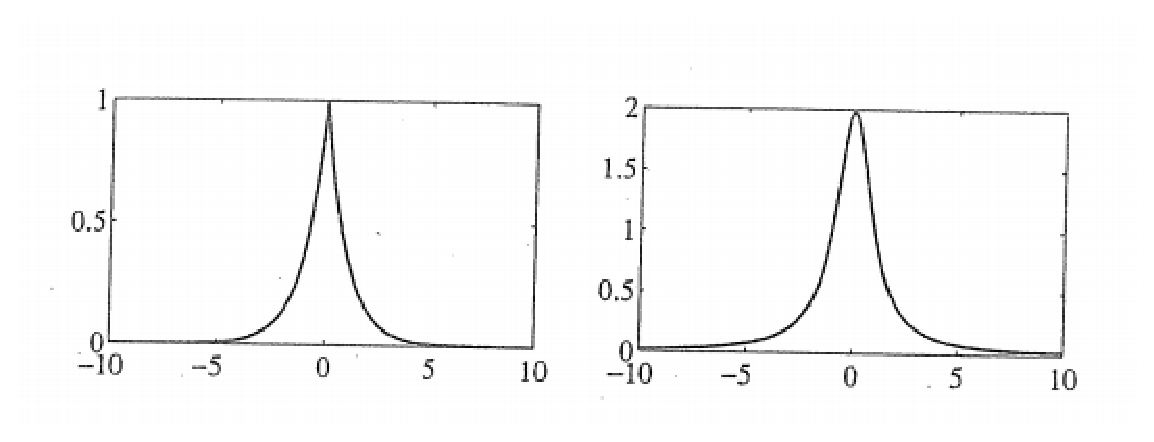
\includegraphics[width=0.7\linewidth]{TeX_files/Part02/chapter05/image/1}
      	\caption{Autocorrelation $ R_{x}(\tau) $ and spectral density function $ S_{x}(\omega) $ for a GaussMarkov process with $ \sigma=1 $ and $ \alpha=1 $.}
      \end{figure}
      
	      	We assume the noise  $ \varepsilon_{\tau} $ is normally distributed with zero mean and calculate the variance:
	      	\begin{equation}\label{5.20}
	      	\begin{aligned}
	      E\left\lbrace\epsilon_{\tau}^{2} \right\rbrace &=E\left\lbrace(x(t+\tau)-e^{-\alpha|\tau|x(t)})^{2} \right\rbrace\\
	      &=E\left\lbrace x(t+\tau)^{2}-2e^{-\alpha|\tau|}x(t+\tau)x(t)+e^{-2\alpha|\tau|}x(t)^{2}\right\rbrace \\
	      &=\sigma^{2}-2\sigma^{2}e^{-\alpha|\tau|} +\sigma^{2}e^{-2\alpha|\tau|}\\
	      &=\sigma^{2}(1-e^{-2\alpha|\tau|}) 
	      	\end{aligned}
	      	\end{equation}
	      	 
	     
	       We assumed that $ \epsilon_{\tau} $ is independentof $ x(t) $.This process is called an autoregression.
	       If $ \epsilon_{k}  $ are i.i.d. and we sample at $k = 1, 2, 3,...$the process is described as 
	       \begin{equation}\label{5.21}
	        x_{k}=px_{k-1} +\epsilon_{k}
	       \end{equation}
	       
	       
	       where $ p=e^{-\alpha} $ when the sampling interval is $ \tau=1 $ .
	       
	       The inverse transform of $ S_{x}(\omega) $ the spectral densityreconstructs the autocorrelation:
	      	\begin{equation}\label{5.22}
	      	R_{x}(\tau)=\frac{1}{2\pi}\int_{-\infty}^{+\infty}S_{x}(\omega)e^(j\omega\tau)d\omega
	      	\end{equation}
	       
	      	
	      	For $ \tau=0 $ this is
	      	\begin{equation}\label{5.23}
	      	 R_{x}(0)=E\left\lbrace x^{2}(t) \right] =\frac{{1}{2\pi}}\int_{-\infty}^{+\infty} s_{x}(\omega)d\omega
	      	\end{equation}
	       
	      	
	      	As $ R_{x}(\tau)=R_{x}(-\tau) $ we also get $ S_{x}(\omega)=S_{x}(-\omega) $ ,so the power spectral density function is a symmetric function in $ \omega $ . 
	      	
	      	\textbf{Example 5.5} (Gauss-Markov process) We consider the spectral function (5.19)
	      	
	      	\[ S_{x}(\omega)=\frac{2\sigma^{2}\alpha}{\alpha^{2}+\omega^{2}} \]
	      	
	      	Using (5.23) we should recover $ \sigma^{2} $.So we perform the integration:
	      	\begin{equation*}
	      	\begin{aligned}
	      	E\left\lbrace x^{2}\right\rbrace&=\frac{1}{2\pi}\int_{-\infty}^{+\infty}\frac{2\sigma^{2}\alpha}{\alpha^{2}+\omega^{2}}d\omega \\
	      	&= \frac{\sigma^{2}\alpha}{\pi}\left\lbrace \frac{1}{\alpha}\arctan(\frac{\omega}{\alpha}) \right\rbrace_{-\infty}^{+\infty} =\sigma^{2}
	      	\end{aligned}
	      	\end{equation*}
	      	 
	      	Taking the inverse Fourier transform of the Fourier transform we have recovered the original function. 
	      	
	      	\begin{figure}[h]
	      		\centering
	      		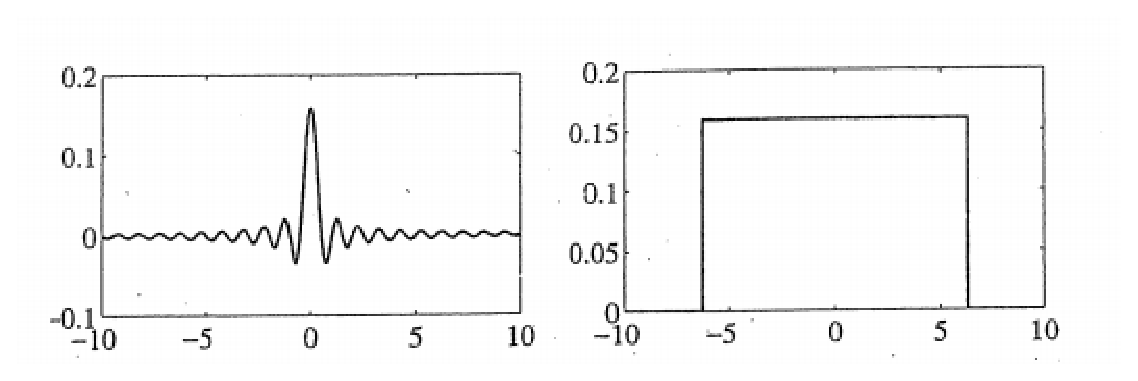
\includegraphics[width=0.7\linewidth]{TeX_files/Part02/chapter05/image/2}
	      		\caption{ Autocorrelation $ R_{x}(\tau) $ and spectral density function $ S_{x}\omega) $ for bandlimited white noise.}
	      	\end{figure}
	      	
	      
	      	
	      	We should like to commenton the interpretation of the power spectral density.White noise is similar to the buzz in the radio and it contains all tones (frequencies). Its power spectral density function is $ S_{x}\omega) $  =constant. On the contrary the power spectral density of a pure cosine waveform has the delta function (actually two delta functions, at $ +\omega $ and $ -\omega $) as power spectral density. The spectral density reflects the composition of frequencies in the signal $ x(t) $ .The following example discusses the subject in a little detail. 
	      	
	      	\textbf{Example 5.6} Which autocorrelation function corresponds to a constant power spectral density $ S_{0} $ from $ -\infty $ to  $ +\infty $ ? The power is distributed uniformly over all frequencies. In analogy to the case of white light such a random process is called white noise:
	      	
	      	$ R_{x}(\tau) =\frac{1}{2\pi}\int_{-\infty}^{+\infty}S_{0}e^{-j\omega\tau}d\omega=S_{0}\delta(\tau) $ informally
	      	
	      	At $ \tau=0 $ , the Dirac delta $ \delta(\tau) $ yields $ R_{x}=S_{0}\delta(0)=\infty $. This is $ E\left\lbrace (x(t))^{2}\right\rbrace  $. Thus white noiseis an idealized process.
	      	
	      	Another characteristic of sound is the bandwidth. Often the bandwidth of the noise is made wide compared to the bandwidth of the system. We define a bandlimited white noise as constant in a finite range of frequencies and zero elsewhere:
	      	
	      	\[ S(\omega) =\{ _{0,for|\omega|>2\pi W}^{A,for|\omega|<2\pi W} \]
	      	
	      	$W$ is the physical bandwidth in Hertz. The autocorrelation of $ S(\omega) $ is the inverse transform of this box function, which produces the sine function $ \frac{\sin x}{x} $ :
	      	
	      	\[ R(\tau)=2WA\frac{\sin (2\pi W \tau)}{2\pi W \tau}\]
	      	
	      	This is not bandlimited. It is impossible for both $ S(\omega) $  and $ R(\omega) $ to be supported on finite intervals. Heisenberg’s Uncertainty Principle gives a precise limitation $ \sigma_{S}\sigma_{R} >\frac{1}{2} $ on their variances. 
	      	
	      	Both the autocorrelation and spectral density functions for bandlimited white noise are sketched in Figure 5.2. The function $ R_{x}(\tau) $ is zero for $ \tau=\frac{1}{2W},\frac{2}{2W},\frac{3}{2W}... $ Thus if the process is sampled at the Nyquistrate of 2W samples/sec, the resulting discrete random variables are uncorrelated.Since this usually simplifies the analysis,the white bandlimited assumption is frequently made.
	      	  
	      	  
	      	  \[ \textbf{Table 5.1} \quad System models of continuous random process \] 
	      	  \[ \begin{tabular}{lcr}
	      	  \hline
	      	   Process\quad type & $ Autocorrelation\quad R_{x}(\tau) $ & $ Power \quad spectral \quad density S_{x}(\omega) $ \\
	      	  \cline{1-3}
	      	  White \quad noise &$  \sigma^{2}\delta(\tau) $  & $ \sigma^{2} $(constant)\\
	      	  \cline{1-3}
	      	  Random \quad walk&undefined&$ \sigma^{2}/\omega^{2} $\\
	      	  \cline{1-3}
	      	  Random \quad constant&$ \sigma^{2} $&$ 2\pi\sigma^{2}\delta(\omega) $\\
	      	  \cline{1-3}
	      	  Exponenitially\quad correlated &$ \sigma^{2}e^{-\alpha|\tau|} $,where\quad$  1/\alpha= $&$ \frac{2\sigma^{2}\alpha}{\omega^{2}+\alpha^{2}} $\\
	      	  \cline{1-3}
	      	 $ or\quad Gauss-Markov  $& $ correlation\quad time $& $ \quad $ \\
	      	  \hline
	      	  \end{tabular} \]      	  
	      	  Not a stationary process, hence undefined $ R_{x}(\tau) $.
	      	  
	      	  
	      	  
	      	